\chapter{He Made \$7M/Year And Paid Zero Taxes}

This chapter follows the School of Hard Knocks interview with Carlton Dennis as curated by LazyingArt LLC through Video2Book. The subject is not an abstract theory of taxation, but a sequence of claims, examples, and mechanisms: high income, low reported tax, paper losses, depreciation, leverage, documentation, and the speed with which experienced business owners act when a tax problem appears.

\section{The Claim That Creates the Puzzle}

The lecture opens with a deliberately startling contrast. Carlton is introduced through a viral Ferrari interview: he says he owns a consulting firm, has been an entrepreneur for six years, and made just over \$7.1 million in a single year. The hook is not only the income number. It is the claim that he had already offset his taxes for the year and then bought the Ferrari in cash.

In the longer interview, the numbers become more explicit. Carlton says that in 2023 he made about \$7.1 million, paid \$0 in federal taxes, and paid \$26,000 in state taxes. He then says that in 2024 the business had crossed \$11.5 million and was on pace to pay less than \$92,000 in total taxes.

\begin{align}
I_{2023} &\approx \$7.1\text{ million},\\
T_{\mathrm{fed},2023} &= \$0,\\
T_{\mathrm{state},2023} &= \$26{,}000,\\
I_{2024} &> \$11.5\text{ million},\\
T_{\mathrm{total},2024} &< \$92{,}000.
\end{align}

Those equations are not tax law. They are the interview's stated puzzle. The chapter has to keep them as claims made by the speaker, because the rest of the conversation is organized around the question they raise.

\subsection{Question \& Answer}

\paragraph{Question.}
How can someone report very high income and still claim a near-zero federal tax bill?

\paragraph{Answer.}
Carlton's answer is that there is no single trick. He names three recurring categories: income shifting, depreciation through real estate, and charitable structure through a private family foundation. His explanation is that the tax bill is not defeated by pretending income does not exist, but by creating deductions, losses, and structures that change what remains taxable.

\section{Three Mechanisms, Not One Trick}

Carlton first frames his approach as legal and rule-based. When the host asks whether the IRS could come after him, he says that everything is by the book and that he is not afraid to use the tax code. The three mechanisms he lists are:

\begin{enumerate}
\item income shifting strategies, described as taking money off the tax return;
\item depreciation, especially paper losses from real estate;
\item philanthropy through a private family foundation.
\end{enumerate}

The important distinction is between a cash loss and a paper loss. A cash loss means money actually went out and was not recovered. A paper loss, in Carlton's use here, means a deduction created by depreciation or related tax accounting. The asset may still exist; the tax return records a loss.

If \(I\) is reportable income and \(L_{\mathrm{paper}}\) is a paper loss, the simplified arithmetic of the interview is:

\begin{equation}
I_{\mathrm{taxable}} \approx I - L_{\mathrm{paper}}.
\end{equation}

That is the core mathematical motif of the lecture. The rest of the interview keeps returning to the same shape: find income, find a permitted offset, document the reason, and redeploy what would otherwise have gone to tax.

\section{Short-Term Rentals As Active Loss Machinery}

The first concrete mechanism is real estate, and more specifically short-term rentals. Carlton says that a full-time W-2 or 1099 taxpayer should look at short-term rentals because, in his account, managing the rental for 100 hours can help make it an active business. He adds another condition: tenants stay in the property seven days or less. Under those conditions, he says, the taxpayer can perform a cost segregation study and create a paper loss that may offset W-2 or 1099 income.

The stated rule-conditions can be recorded compactly:

\begin{align}
\mathrm{STR} &:\quad \text{average stays of }7\text{ days or less},\\
H_{\mathrm{management}} &\geq 100\text{ hours},\\
\text{cost segregation} &\longrightarrow \text{accelerated depreciation},\\
\text{accelerated depreciation} &\longrightarrow L_{\mathrm{paper}}.
\end{align}

The host then asks about someone who is earlier in the journey: perhaps making the first six figures, with thinner margins, and without enough capital to buy real estate. This is an important transition. The lecture does not stay with advanced real estate machinery; it backs up to the first structural decision a new business owner may face.

\subsection{Question \& Answer}

\paragraph{Question.}
What if the person does not yet have enough money to start buying real estate?

\paragraph{Answer.}
Carlton answers with entity structure first. He says many self-employed people begin as sole proprietors or single-member entities, which may be fine until they cross roughly \$50,000 to \$60,000. After that, he recommends looking at an S corporation so that the owner can pay a salary and avoid self-employment tax on some remaining business profit, as he describes it.

\begin{align}
t_{\mathrm{SE}} &= 15.3\%,\\
\text{threshold for review} &\approx \$50{,}000\text{--}\$60{,}000,\\
\text{S corporation planning} &:\quad
\text{salary}+\text{remaining profit}.
\end{align}

This is not presented as a universal command. In the interview, it is a beginner-oriented sequence: first structure the entity, then identify legitimate expenses that were missed, then graduate to larger deductions and investment structures.

\section{Speed, Documentation, And Audit Defense}

The host next asks for the difference between middle-class and wealthy approaches to taxes. Carlton's answer is speed. Wealthy clients, as he describes them, ask where the money should move, when to set up the foundation, and where to send the wire. Hesitant clients, by contrast, may remain in analysis paralysis until the chance to act has passed.

But the next story shows that speed alone is not the real standard. Carlton describes a client facing an audit over a \$1 million vehicle deduction. The vehicle turns out to be a yacht. The reason it matters to the business, according to the story, is that she is a real estate agent who shows athletes and entertainers coastal property from the water. The audit defense rests on documentation: captain's logs, photos, expenses from the profit-and-loss statement, and a business-purpose argument.

The rule he invokes is the ordinary, necessary, and reasonable business deduction test, which he attributes in the interview to code section 162A. The transcript may be imprecise here; the common reference is section 162(a). For the notes, the point is not the exact citation but the structure of the defense:

\begin{equation}
\text{Deduction survives}
\quad\Longleftarrow\quad
\text{business purpose}+\text{ordinary/necessary fit}+\text{documentation}.
\end{equation}

That episode prevents the chapter from becoming a list of hacks. The mechanism must be attached to a business reason and supported by records.

\section{Cars, Depreciation, And Reinvestment}

The interview then moves outside to the cars. This could look like a lifestyle interruption, but in the lecture's rhythm it is another worked example. Carlton agrees that cars are depreciating assets. His point is that depreciation itself can become part of the tax arithmetic.

He says he took 100\% bonus depreciation on one car and saved about \$92,000 in taxes. He then says that the \$92,000 was reinvested into a multifamily property in Texas producing about \$1,400 per month in cash flow.

\begin{align}
\text{tax saving} &\approx \$92{,}000,\\
\text{reinvestment} &\longrightarrow \text{Texas multifamily property},\\
\text{monthly cash flow} &\approx \$1{,}400/\text{month}.
\end{align}

The G-Wagon example adds conditions. Carlton says the vehicle qualifies because the gross vehicle weight rating is over 6,000 pounds and the vehicle is used more than 50\% for business. He mentions Section 179 and Section 168(k), and he notes that bonus depreciation was 100\% in 2022, moved to 80\% in 2023, and was 60\% in 2024 at the time of the interview.

\begin{align}
\mathrm{GVWR} &> 6{,}000\ \mathrm{lb},\\
\text{business use} &> 50\%,\\
\text{deduction path} &\sim \S 179+\S 168(k).
\end{align}

The host asks how someone could afford a G-Wagon. Carlton responds with leverage. His example is a business owner making \$200,000, putting \$20,000 down on a qualifying vehicle, and claiming a roughly \$200,000 write-off. If that person might otherwise have paid about \$50,000 in taxes, then the arithmetic he emphasizes is:

\begin{align}
I &= \$200{,}000,\\
W_{\mathrm{vehicle}} &\approx \$200{,}000,\\
T_{\mathrm{avoided}} &\approx \$50{,}000,\\
D_{\mathrm{cash}} &= \$20{,}000,\\
\Delta &= T_{\mathrm{avoided}}-D_{\mathrm{cash}}
       = \$50{,}000-\$20{,}000
       = \$30{,}000.
\end{align}

The lesson he draws is that the remaining \$30,000 can be redeployed into a cash-flowing asset or back into the business. The claim is not that a car stops depreciating. It is that the tax effect of depreciation can be converted into working capital.

\section{Leverage As Buying Power}

The debt discussion follows naturally from the vehicle example. Carlton distinguishes bad debt from good debt. Bad debt is consumer debt, credit-card debt, and high-interest-rate debt. Good debt, in his framing, is asset-backed borrowing, especially real estate debt, where the borrower controls an appreciating or income-producing asset and may later borrow against it through a refinance or HELOC.

The conceptual update rule is simple:

\begin{equation}
\text{buying power}
\quad\text{increases when}\quad
\text{retained cash}+\text{credit access}
\quad\text{increase together}.
\end{equation}

The interview then shifts from the ethics of debt to the mechanics of access. Carlton says the best way to get access to credit is to use credit and build relationships with bankers. Deposits and banking relationships may lead to a private banker, and the private banker understands the business well enough to evaluate requests for debt.

This section sets up the final whiteboard calculation. The reason leverage matters is that the taxpayer in the example does not need \$500,000 in cash. He needs enough cash to control the asset and enough credit to finance the rest.

\section{Whiteboard Walkthrough: Turning \$500,000 Into A Paper Loss}

The lecture culminates in a whiteboard example. The host asks for a walkthrough for someone making \$100,000 a year. Carlton takes that number as W-2, 1099, or entrepreneurial income, then builds the rental-property example around it.

\begin{figure}
\centering

\includegraphics[width=\linewidth]{lecture_04_figure_02.png}
\caption{Carlton Dennis writes the short-term rental tax example on the board. The visible board notes include the short-term rental condition, the seven-day-or-less stay rule, the 100-hour management note, and the \$500,000 property example.}
\label{fig:str-board}
\end{figure}

The clean reconstruction of the example is:

\begin{align}
I &= \$100{,}000,\\
P &= \$500{,}000,\\
D &= \$100{,}000,\\
L &= P-D=\$500{,}000-\$100{,}000=\$400{,}000.
\end{align}

Here \(I\) is the income to be offset, \(P\) is the property value, \(D\) is the saved cash or down payment, and \(L\) is the loan. The property is then listed as a short-term rental. The stated operating requirements are:

\begin{align}
\mathrm{STR} &= 7\text{ days or less},\\
H_{\mathrm{management}} &= 100\text{ hours}.
\end{align}

Carlton then says that a cost segregation study can yield, on average in this example, 20\% of the building's purchase price as a year-one tax write-off. The 20\% value is transcript-supported rather than fully legible in the board frame, so it should be read as the spoken calculation.

\begin{align}
L_{\mathrm{paper}}
  &\approx 20\%\times P\\
  &=0.20\times \$500{,}000\\
  &=\$100{,}000.
\end{align}

Now the central arithmetic closes:

\begin{align}
I_{\mathrm{taxable}}
  &\approx I-L_{\mathrm{paper}}\\
  &=\$100{,}000-\$100{,}000\\
  &\approx \$0.
\end{align}

That is the lecture's most explicit derivation. It also explains why Carlton keeps returning to debt. Without borrowing, the example requires \$500,000 in cash. With leverage, the taxpayer controls a \$500,000 property using \$100,000 saved and \$400,000 of other people's money.

A narrow flowchart preserves the mechanism without turning it into a sprawling diagram.

\begin{figure}
\centering
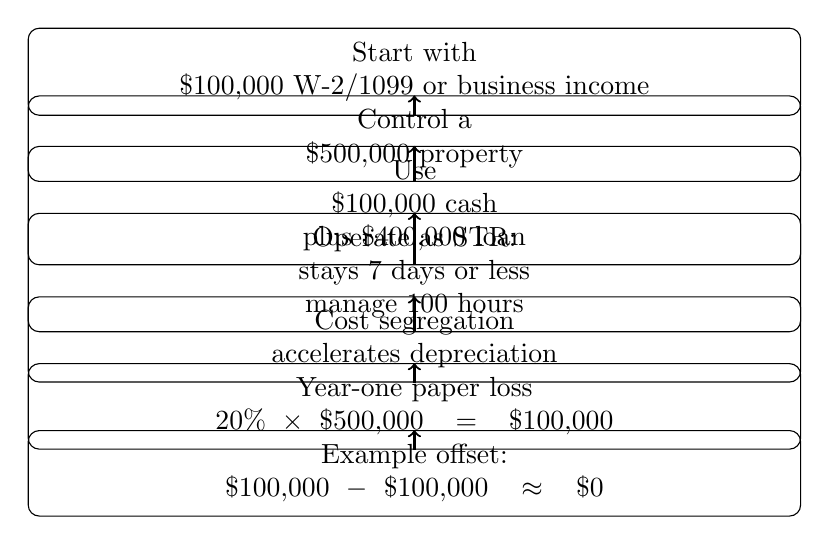
\begin{tikzpicture}[
  node distance=0.85cm,
  every node/.style={draw, rounded corners, align=center, text width=0.78\linewidth, inner sep=5pt},
  arrow/.style={->, thick}
]
\node (a) {Start with\\ \(\$100{,}000\) W-2/1099 or business income};
\node (b) [below of=a] {Control a\\ \(\$500{,}000\) property};
\node (c) [below of=b] {Use\\ \(\$100{,}000\) cash\\ plus \(\$400{,}000\) loan};
\node (d) [below of=c] {Operate as STR:\\ stays \(7\) days or less\\ manage \(100\) hours};
\node (e) [below of=d] {Cost segregation\\ accelerates depreciation};
\node (f) [below of=e] {Year-one paper loss\\ \(20\%\times \$500{,}000=\$100{,}000\)};
\node (g) [below of=f] {Example offset:\\ \(\$100{,}000-\$100{,}000\approx \$0\)};

\draw[arrow] (a) -- (b);
\draw[arrow] (b) -- (c);
\draw[arrow] (c) -- (d);
\draw[arrow] (d) -- (e);
\draw[arrow] (e) -- (f);
\draw[arrow] (f) -- (g);
\end{tikzpicture}
\caption{A pocket-size reconstruction of the short-term rental and cost-segregation example shown in the board frame.}
\label{fig:str-flow}
\end{figure}

The final tactic in the interview is the Augusta rule. Carlton describes it as a rule allowing a homeowner to rent out a primary residence for 14 days or less and not pay tax on the rental income for those days. For business owners, he describes an S corporation renting the owner's primary residence for meetings, deducting the rent at the company level, and sending rent back to the individual.

\begin{equation}
\text{primary-residence rental days}\leq 14
\quad\Longrightarrow\quad
\text{rental income excluded, as described in the interview}.
\end{equation}

This is best treated as a compact closing mechanism, not as a second full derivation. The lecture has already done its main arithmetic on the whiteboard.

\section{Summary}

The lecture begins with a spectacle, but its structure is mathematical. The central object is not the Ferrari; it is the offset:

\begin{equation}
\text{taxable income in the example}
\approx
\text{income}
-
\text{documented deductions or paper losses}.
\end{equation}

Carlton's interview supplies a sequence of mechanisms: income shifting, depreciation, foundations, short-term rentals, entity structure, ordinary-and-necessary deduction logic, vehicle depreciation, leverage, banking relationships, and the Augusta rule. The most concrete worked example is the \$500,000 short-term rental: \$100,000 cash, \$400,000 debt, short stays, 100 hours of management, cost segregation, and a claimed \$100,000 paper loss.

The notes should preserve the caution as much as the arithmetic. These are interview claims and examples, not a universal tax prescription. The durable lesson for the larger book is that wealth is not only income; it is control over structures, assets, timing, documentation, and access to capital.